\subsection{Bluez : Kernel}

%%%%%%%%%%%%%%%%%%%% HCI %%%%%%%%%%%%%%%%%%%%%%%%%%%%%%%
\begin{frame}
	\begin{columns}[t]
\begin{column}{0.60\linewidth}
	\begin{figure}
		\includegraphics[height=5cm]{img/bluez_kernel_hci.png}
		\caption{Host to Controller Interface}
	\end{figure}
\end{column}
\begin{column}{0.40\linewidth}
	\begin{block}{HCI}
		\begin{itemize}
			\item Queueing
			\item Ordonnancement
		\end{itemize}
		Transport : 
		\begin{itemize}
			\item USB
			\item UART
			\item PCI
			\item SDIO
			\item PCMCIA
		\end{itemize}
	\end{block}
\end{column}
\end{columns}
\end{frame}

%%%%%%%%%%%%%%%%%%%% HCI MGMT %%%%%%%%%%%%%%%%%%%%%%%%%%%%%%%
\begin{frame}[fragile]
	\begin{columns}[t]
\begin{column}{0.60\linewidth}
	\begin{figure}
		\includegraphics[height=5cm]{img/bluez_kernel_hci_sock.png}
		\caption{Management interface}
	\end{figure}
\end{column}
\begin{column}{0.40\linewidth}
	\begin{block}{mgmt socket}
		\begin{itemize}
			\item HCI pour userspace
			\item Remplace hci sockets
		\end{itemize}
	\end{block}
	\begin{block}{Paramètres}
		\begin{Verbatim}[fontsize=\tiny]
- PF_BLUETOOTH
- BTPROTO_HCI
struct sockaddr_hci
 - .hci_family = AF_BLUETOOTH
 - .hci_dev = HCI_DEV_NONE
 - .hci_channel = HCI_CHANNEL_CONTROL
		\end{Verbatim}
	\end{block}
\end{column}
\end{columns}
\end{frame}

%%%%%%%%%%%%%%%%%%%% L2CAP SOCKET %%%%%%%%%%%%%%%%%%%%%%%%%%%%%%%
\begin{frame}[fragile]
\begin{columns}[t]
\begin{column}{0.60\linewidth}
	\begin{figure}
		\includegraphics[height=5cm]{img/bluez_kernel_l2cap_sock.png}
		\caption{L2CAP}
	\end{figure}
\end{column}
\begin{column}{0.40\linewidth}
	\begin{block}{l2cap socket}
		\begin{itemize}
			\item API Socket
			\item - Adresse
			\item - PSM 
		\end{itemize}
	\end{block}
	\begin{block}{Paramètres}
		\begin{Verbatim}[fontsize=\tiny]
- AF_BLUETOOTH
- BTPROTO_L2CAP
struct sockaddr_l2
 - .l2_family = AF_BLUETOOTH
 - .l2_bdaddr = *BDADDR_ANY
 - .l2_psm = htobs(0x1001);
		\end{Verbatim}
	\end{block}
\end{column}
\end{columns}
\end{frame}

%%%%%%%%%%%%%%%%%%%% RFCOMM / BNEP SOCKET %%%%%%%%%%%%%%%%%%%%%%%%%%%%%%%
\begin{frame}[fragile]
\begin{columns}[t]
\begin{column}{0.60\linewidth}
	\begin{figure}
		\includegraphics[height=5cm]{img/bluez_kernel.png}
		\caption{RFCOMM, BNEP, etc.}
	\end{figure}
\end{column}
\begin{column}{0.40\linewidth}
	\begin{block}{rfcomm socket}
		\begin{itemize}
			\item API Socket
			\item - Adresse
			\item - Canal
		\end{itemize}
	\end{block}
	\begin{block}{Paramètres}
		\begin{Verbatim}[fontsize=\tiny]
- AF_BLUETOOTH
- BTPROTO_RFCOMM
struct sockaddr_l2
 - .rc_family = AF_BLUETOOTH
 - .rc_channel = 1
 - .rc_braddr = *BRADDR_ANY;
		\end{Verbatim}
	\end{block}

\end{column}
\end{columns}
\end{frame}

